\chapter{Weiterführend}
Weiterführende Verbesserungen der Simulation könnten in folgenden Bereichen implementiert werden:
\begin{itemize}
	\item \textbf{Debuggen:}
	\begin{figure}
		\centering
		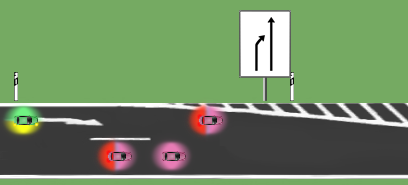
\includegraphics[width=0.7\linewidth]{images/BUG}
		\caption{Rosa Auto ist zuweit gefahren}
		\label{fig:bug}
	\end{figure}

Die Simulation besitzt noch mehrere Bugs. Wenn das Verkehrsvorkommen zu hoch ist, fahren manche Autos einfach über das Hindernis hinweg oder bleiben davor stehen, erkennen aber keine Lücke mehr. Das Problem dabei ist, dass die Fahrzeuge auf der rechten Seite das Fahrzeug noch erkennen und bremsen um dieses reinzulassen. Dadurch kommt es zu unnötigem und realtitätsfernem Rückstau.
Auch der Fahrbahnwechsel ist noch nicht perfekt implementiert. Das Fahrzeug erkennt, wenn es auf der stärker befahrerenen Spur ist und wechselt auf die andere Fahrbahn, jedoch ist dieser Wechsel nicht immer sinnvoll.
\item \textbf{Ein weiteres Verfahren:}\\
Es wäre interessant ein Verfahren zu entwickeln was davon aus geht, dass nur autonome Fahrzeuge beteiligt sind. So könnten aufgrund der Kommunikation zwischen den Fahrzeugen statt Lücken suchen zu lassen, Lücken  gebildet werden, welche dann dem jeweiligen Fahrzeug zugewiesen werden. Diese Verfahren dürfte das Effektivste sein, jedoch frühestens in 20 Jahren von Bedeutung.

\item \textbf{Eine dritte Spur:}\\
Die Effektivität eines Einfädelungsverfahrens ist abhängig von der Anzahl der Spuren. Wenn die Fahrbahn von drei auf zwei Fahrbahnen verengt wird, verhält sich der Verkehr anders, als wenn aus zwei eine Fahrbahn wird. Es gibt viel mehr Platz und es gibt zwei Spuren welche die Engstelle passieren, wodurch der Verkehrsfluss wahrscheinlich besser ist.

\item \textbf{Weitere Fahrzeugarten:}\\
Die Simulation enthält nur eine Art von Fahrzeug. Diese hat eine einheitliche Länge von 4,5\,m und die Breite wird nicht betrachtet. Es kommt jedoch vor, dass in Baustellen die linke Fahrspur nur für Fahrzeuge bis 2,1\,m freigegeben ist.
Zudem wäre es interessant den Einfluss von LKWs oder Wohnwagen auf das Reißverschlussverfahren zu untersuchen.

\item \textbf{Mehr Fahrertypen:}\\
Um eine aussagekräftige Simulation zu erhalten, reicht es aus alle Fahrer in die Kategorien aggressiv, neutral, und passiv, zu unterteilen. In der Realität hat jedoch jeder Fahrer seinen individuellen Fahrstil. Deshalb wäre es interessant, noch mehr Fahrertypen zu ergänzen und detaillierter in ihren Eigenschaften zu beschreiben.

\item \textbf{Verhalten bei Unfällen:}\\
In der derzeitigen Version werden Unfälle zur Kenntnis genommen, aber nicht beachtet. Wenn Autos kollidieren wird lediglich eine Statusmeldung angezeigt, die Geschwindigkeit wir auf 0\,$ \frac{\text{km}}{\text{h}} $, jedoch fahren die Fahrzeuge danach ganz normal weiter.

\item \textbf{Unterschiedliche Gegebenheiten:}\\
Es macht einen Unterschied, ob ein Reißverschlussverfahren auf der Autobahn oder in der Stadt eingesetzt wird, da die Anfangsgeschwindigkeiten unterschiedlich sind und in der Stadt auch Ampeln zu berücksichtigen sind.\\
Zudem macht es einen Unterschied, ob die Verengung Aufgrund einer Baustelle oder eines Unfalls entsteht. Im Falle eines Unfalls könnte man zusätzlich eine Rettungsgasse simulieren.
\end{itemize}